\documentclass{article}

% if you need to pass options to natbib, use, e.g.:
% ©PassOptionsToPackage{numbers, compress}{natbib}
% before loading nips_2016
%
% to avoid loading the natbib package, add option nonatbib:
% \usepackage[nonatbib]{nips_2016}

\usepackage[final]{nips_2016}

% to compile a camera-ready version, add the [final] option, e.g.:
% \usepackage[final]{nips_2016}

\usepackage[utf8]{inputenc} % allow utf-8 input
\usepackage[T1]{fontenc}    % use 8-bit T1 fonts
\usepackage{hyperref}       % hyperlinks
\usepackage{url}            % simple URL typesetting
\usepackage{booktabs}       % professional-quality tables
\usepackage{amsfonts}       % blackboard math symbols
\usepackage{amssymb}
\usepackage{amsmath}
\usepackage{bbm}
\usepackage{nicefrac}       % compact symbols for 1/2, etc.
\usepackage{microtype}      % microtypography
\usepackage{caption}
\usepackage{float}
\usepackage{graphicx}
\usepackage{subfig}
\usepackage{wrapfig}

\graphicspath{ {./} }

\title{DeepRAGE: predicting genome-wide gene expression with promoter sequences and transcription factor expression levels}

% The \author macro works with any number of authors. There are two
% commands used to separate the names and addresses of multiple
% authors: \And and \AND.
%
% Using \And between authors leaves it to LaTeX to determine where to
% break the lines. Using \AND forces a line break at that point. So,
% if LaTeX puts 3 of 4 authors names on the first line, and the last
% on the second line, try using \AND instead of \And before the third
% author name.

\author{
  Boxiang Liu \\
  Department of Biology\\
  \texttt{bliu2@stanford.edu} \\
  \And
  Salil Bhate \\
  Department of Bioengineering\\
  \texttt{bhate@stanford.edu} \\
  \AND
  Scott Longwell \\
  Department of Bioengineering\\
  \texttt{longwell@stanford.edu} \\
  \And
  Tyler Shimko \\
  Department of Genetics\\
  \texttt{tshimko@stanford.edu} \\
  \And
  Anshul Kundaje \\
  Department of Computer Science and Genetics\\
  \texttt{akundaje@stanford.edu} \\
  \And
  James Zou \\
  Department of Biomedical Data Science\\
  \texttt{jamesyzou@gmail.com}
 } 

\begin{document}

\maketitle

\begin{abstract}

The budding yeast \textit{Saccharomyces cerevisiae} possesses a relatively simple transcriptional regulatory system that lends itself to both experimental and computational dissection. Given the simple architecture governing transcriptional regulation in this organism, computational models aiming to predict gene expression levels in varying environmental conditions have generally performed well in comparison to more complex organismal models. However, the majority of these computational models have not yet taken advantage of deep neural network (DNN) techniques, which represent a possible significant improvement in prediction accuracy. Furthermore, the interpretation of DNN models has the potential to yield insights into relationships between regulatory elements and promoter sequences and the interactions of multiple regulatory elements binding at the same promoter. Here, we present a novel DNN architecture called deep regulatory annotation of gene expression (deepRAGE) to predict the expression levels of all genes in the yeast genome using measured expression levels of all regulatory elements and the sequence of the promoter directly upstream of each gene. We find that our model performs well against an existing gene expression dataset and accurately learns experimentally-validated regulatory element/promoter relationships.
  
\end{abstract}

\section{Introduction}

The faithful prediction of gene expression levels based on primary DNA sequence is a critical milestone toward fully comprehending cellular dynamics. Modulation of expression levels allows the host cell to react and adapt to its environment, enhancing the ability of the cell to survive in the face of constantly-evolving pressures. Many factors have the ability to influence gene expression levels including environmental stresses, the cell cycle, and stochastic fluctuations of cellular state. The cell can perceive these changes using molecular sensors, which further transmit information through molecular signaling cascades, ultimately resulting in activation of transcriptional regulatory elements. These regulatory elements have the capacity to bind genomic DNA in a specific manner and activate or repress expression of genes to control the cell's response to the sensed change in state.

Expression levels can, therefore, be conceptualized at the most basic level as the output of a complex function of regulatory element/DNA interactions. Specifically, transcription factors, proteins that bind DNA and have the ability to activate or repress transcription of downstream genes, tend to preferentially bind certain DNA sequences termed “motifs.” However, expression of the downstream gene relies on both the presence of these motifs in the gene’s promoter sequence as well as the expression levels of the regulatory elements themselves. Without expression of the required regulatory element, the presence of the desired motif will fail to impact expression levels. Additionally, transcription factors exhibit what is known as "combinatorial control" over gene expression levels \cite{Kato:2004is}. In this scenario, the role of the transcription factor to either promote or repress gene expression is dictated by the presence of other transcription factors binding in the promoter region alongside it.

The budding yeast \textit{Saccharomyces cerevisiae} represents an ideal model organism within which to learn the grammar of regulatory element/promoter interactions. The transcriptional regulatory architecture of this yeast species is relatively simple, with the expression of the majority of genes being governed primarily by interactions between regulatory elements and the promoter sequence directly upstream of the gene. There exist very few long range genomic interactions in \textit{S. cerevisiae} such as those that would complicate such a project in higher-order organisms \cite{Dobi:2007eo}. We also expect relatively few binding interactions to have large effects on downstream transcription, as previous work has shown the overwhelming majority of promoters to be bound by fewer than 5 regulatory elements \cite{Lee:2002jm}.

While machine learning techniques have previously been applied to the task of predicting gene expression levels, these strategies have yet to take advantage of nascent developments in deep neural networks (DNNs). Here, we present a DNN architecture that is capable of predicting gene expression levels given the expression level of the complete set of \textit{S. cerevisiae} regulatory elements as well as the 1 kilobase sequence directly upstream of the transcription start site. This model takes advantage not only of count and spatial relationships between sequence motifs in the promoters of the individual genes, but also the amount of each regulatory element available to interact with those motifs. We demonstrate that under certain circumstances, our model achieves accuracy on par with leading algorithms employing classical machine learning techniques. Furthermore, since the sequence specificities of most DNA-binding regulatory elements have been experimentally validated \cite{deBoer:2011ic}, we show that we can use existing information about regulatory element binding specificities to interpret the results from out model.

Overall the application of DNNs to the prediction of gene expression levels represents a marked advance in the field of computational biology. Our model serves as a proof-of-principle, demonstrating that it is possible to achieve accuracy similar to leading models quite rapidly using DNN architectures.

\section{Related Work}

Understanding the regulation of gene expression is a central problem in computational biology. Traditional approaches use gene knockout or knockdown to experimentally verify the regulatory role of specific transcription factor, and mutagenesis to probe the binding affinity change of cis-regulatory elements. The advent of microarray and next-generation sequencing enabled researchers to probe the gene expression in a genome-wide fashion, enable simultaneous measurement of thousands to tens of thousands of regulators and genes being regulated. In simple model organisms such as yeast \textit{S. cerevisiae}, several efforts has been made to predict the regulation of gene expression across different experimental conditions, by leverage information about regulators and motifs. These studies can be broadly categorized into the following: 1) frequentist approach to identify statistically significant regulatory patterns, 2) Bayesian approaches to calculate the probability of regulatory patterns through probabilistic graphical networks 3) prediction-based approaches which recognizes regulatory patterns to predict expression changes (a review can be found in Middendorf, \textit{et al.}). Here we briefly review the last category as it is the most relevant to this study.

Middendorf, \textit{et al.} uses boosting with a margin-based generalization of decision trees, or alternating decision trees \cite{Middendorf:2004gta}. This model is able to describe the interaction between transcription factors and their binding motifs, but it requires discretizing the outcome. In other words, it predicts expression to be either up- or down-regulated, rather than explicitly predicting expression values. Ruan and colleagues used bi-directional multi-variate regression tree, treating either the conditions or the genes as observations, also predicts discretized gene expression classes\cite{Ruan:2006hl}. The same group also augmented the feature space by including the the chromatin immunoprecipitation (ChIP-chip) data in their package CAGER to perform the same classification task \cite{Ruan:2005dd}. Fröhler and colleagues uses inductive logic programming and additional protein-protein interaction networks to perform the same classification task \cite{Frohler:2007fy}. These studies suggest that information contained in cis-regulatory elements as well as regulator expression is sufficient in prediction of gene regulation.

\subsection{DNN to predict TF binding}
Inspired by recent progress on deep learning, many groups applied convolutional neural network models to predict chromatin accessibility and transcription factor binding. DeepBind uses a CNN to predict RNA and DNA binding sequence specificity \cite{Alipanahi:2015fb}. DanQ tried to improve the prediction accuracy using a CNN and RNN hybrid network \cite{Quang:2016jt}. Basset uses a CNN to predict chromatin accessibility \cite{Kelley:2016bv}. Notably, they show that a multi-task prediction framework (multiple cell times at once) improves the prediction accuracy. These studies suggest that DNNs are good candidate models to predict open chromatin and protein-DNA interaction. In this study, we incorporate a CNN to scan the promoter sequences of each gene and combine this information with a separate network for regulatory gene expression. 

\section{Dataset and Pre-processing}

\textit{S. cerevisiae} is frequently studied, allowing the use of varied experimental data for gene expression. In this study, the experimental data is identical to that used in the initial training of the MEDUSA software package \cite{Kundaje:2007hs}. This dataset queried gene expression levels in yeast through the use of microarray platforms in a variety of environmental conditions. Specifically, three smaller datasets were combined to yield the final, larger dataset. These subset include data regarding \textit{S. cerevisiae} response to environmental stress, DNA-damaging agents, and oxygen sensing and response to hypoxia.

The combined dataset from these experiments contained a total of 6100 genes under 173 experimental conditions and the resulting normalized expression level for each gene under experimental condition (Fig \ref{dataset}). The input portion of this dataset that was fed into the model consisted of collection of gene-experiment pairs, of the form $X$ = ($X_g$, $X_e$). $X_g$ was one thousand base pair promoter sequence for each gene, encoded as one-hot. $X_e$ was the experimental variable, represented as 472-dimensional vectors of log-fold change in expression of transcription factors associated with each experimental condition. The output dataset was the classification of the normalized gene-expression level, sorted into 5 bins. The was a 60-10-30 split among training, validation, and test datasets. Test data could be unseen gene, unseen experiments, or unseen gene/experiment pairs.

\begin{figure}
\begin{center}
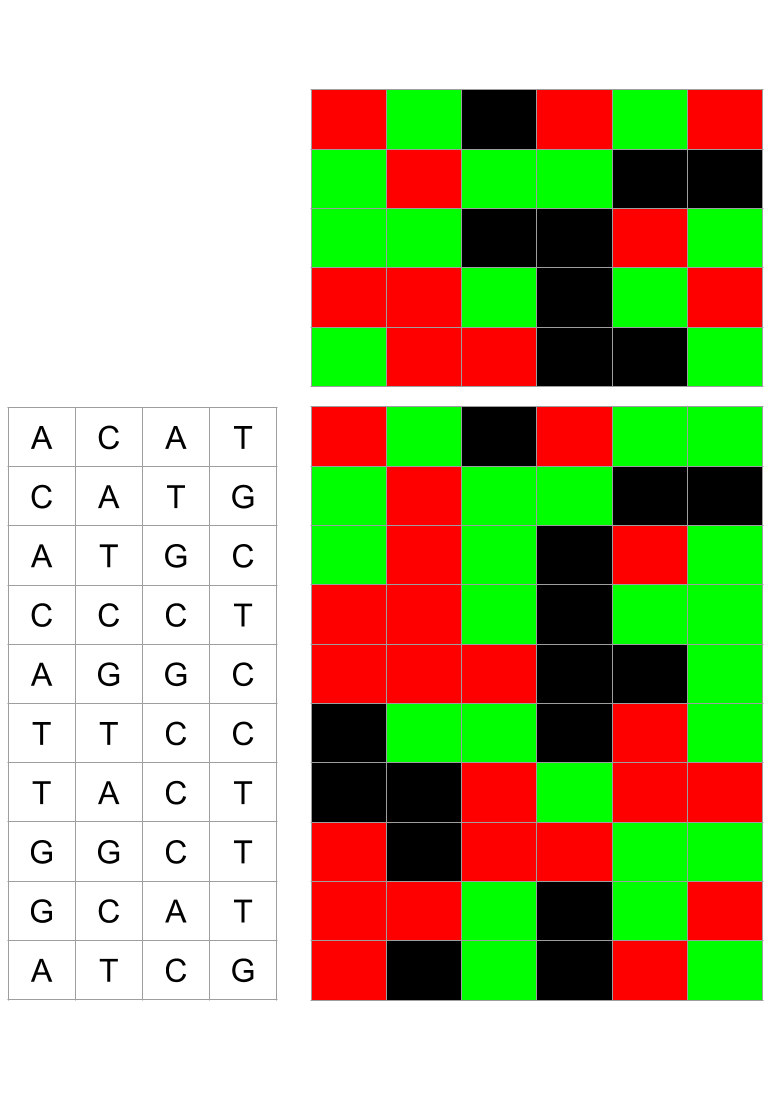
\includegraphics[width=0.45\textwidth]{fig/Dataset.png}
\end{center}
\caption{The data format. Each row of the main matrix represent a gene where as each column represent a condition. Each gene is associated with a unique sequence of promoters and each condition has a unique combination of transcription factor expression levels.}
\label{dataset}
\end{figure}

\section{Methodology}

The dataset consists of two types of data pertaining to different biological interpretations. The promoter sequences is equivalent to matrix in $\{0,1\}^{4 \times 1000}$. Each column of the matrix is a indicator vector representing a neucleotide. In contrast, the transcription factor expression levels are log2 transformed microarray intensities in $\mathbb{R}$. Further, the promoter sequences are gene-specific, whereas the transcription factor expression levels are condition-specific. In the sequence data, short stretches of neucleotide within the promoter (called motifs) determines the binding specificity of transcription factors. Since such short sequences often occur at multiple places across the genome, convolutional networks appear as a natural choice. In contrast, transcription factors does not contain intrinsic spatial patterns. Since several transcriptions factor often act in synergy to bind the same motif in order to activate transcription, it is natural to model their interaction with a fully connected network. The two networks must be combined to leverage information across genes and across conditions. In the subsections, we discuss three ways to do so.


\subsection{Concatenation}

Concatenation is the simplest way to combine the two networks. To concatenate the 2D sequence network and the 1D expression network, we first flatten the sequence network to 1D before combining. The sequence inputs propagate through 2D convolutional layer with ReLu activation. 

\begin{equation} \label{eq1}
x_{ij}=\max \{ 0, \sum_{a=1}^{4} \sum_{b=1}^{l} W_{abj}^{seq} s_{(a)(i+b)} + b^{seq}\}
\end{equation} 

Where $s$ represents sequence input, $W^{seq}$ represents the weight for convolutional filters, $i$ represents the genomic location, $j$ represents filter number, $b^{seq}$ represents the bias, and $l$ represents the filter length. The transcription factor expression inputs propagate through a fully connected network with ReLu activation. 

\begin{equation} \label{eq2}
y=\max \{0, W^{reg}r + b^{reg}\}
\end{equation}

Where $W^{reg}$ and $b^{reg}$ represent the weight and bias for the fully connected layer. We flatten the sequence layer and concatenate both layers. 

\begin{align} \label{eq34}
x' &= [x_{1},x_{2},...,x_{I}] \\
z &= [x',y]
\end{align}

Where $x_{i}$ represent the row i of the matrix $\{ x_{ij} \}$. The concatenation layer propagate through three fully connected layers with ReLu activation. The final layer generate a scalar as the predicted expression value. The entire network is represented as follows in graphical form. 


\begin{figure}[!tbp]
  \centering
  \subfloat[Concatenation]{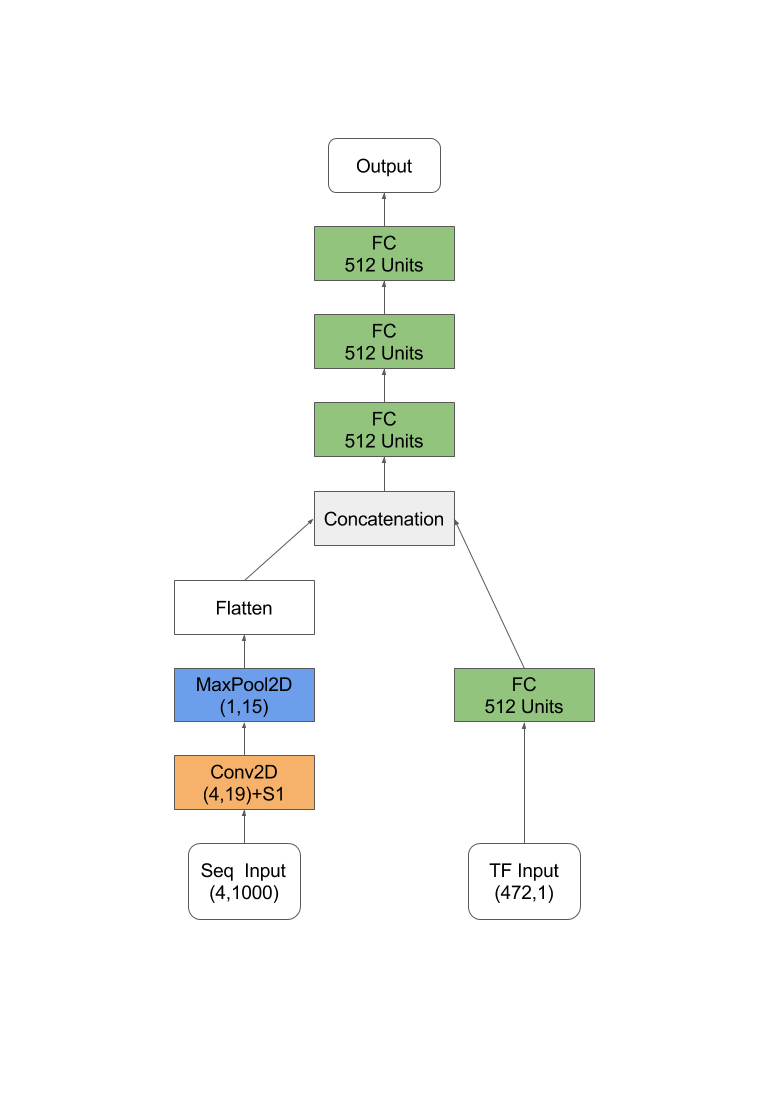
\includegraphics[width=0.3\textwidth]{fig/Architecture_concatenation.png}\label{fig:1a}}
  \hfill
  \subfloat[Tensor Product]{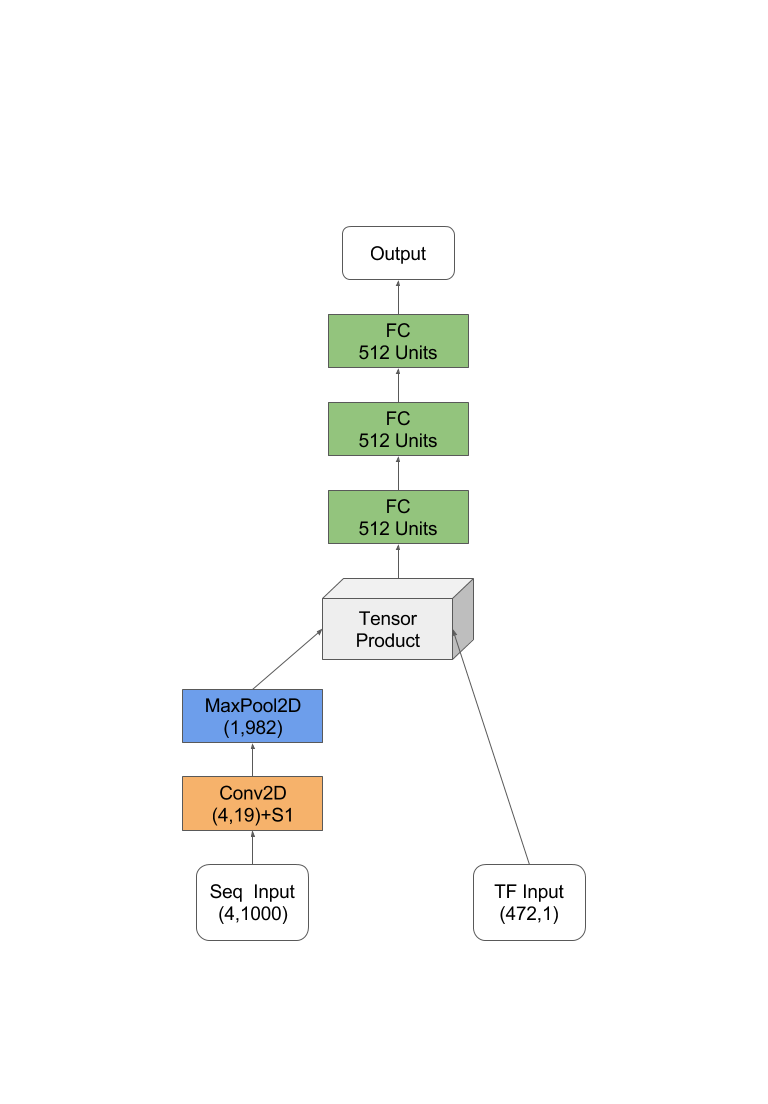
\includegraphics[width=0.3\textwidth]{fig/Architecture_tensor.png}\label{fig:1b}}
  \subfloat[Concatenation-RNN]{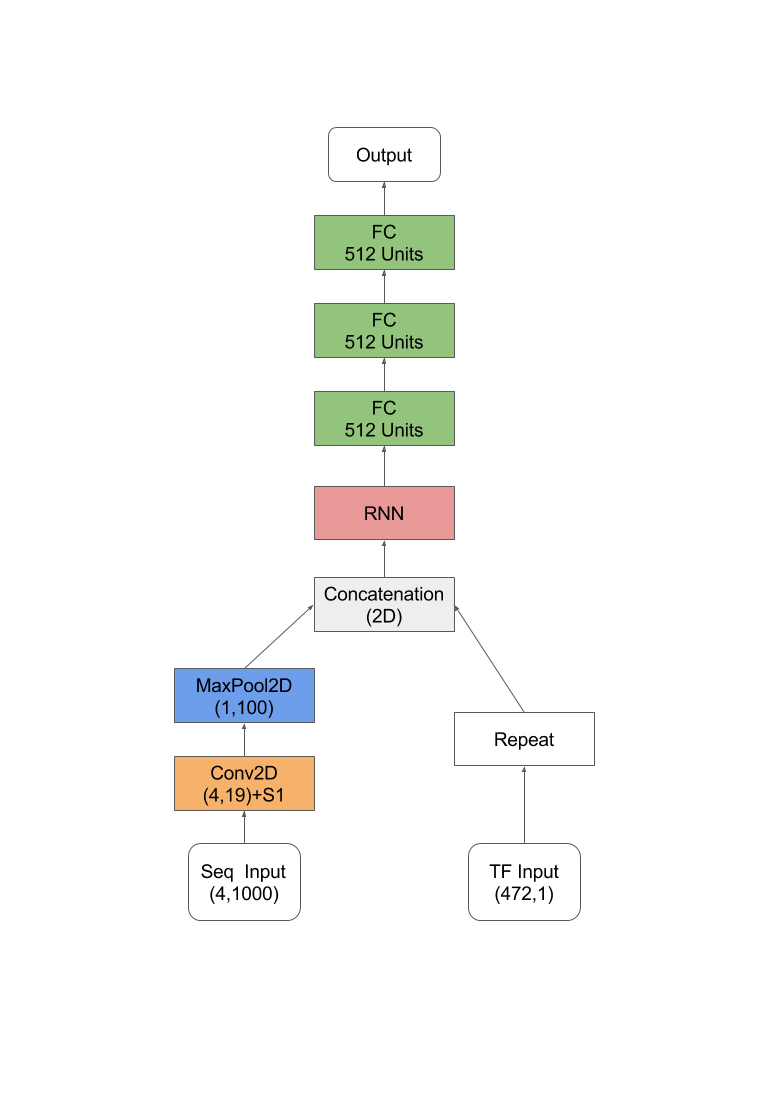
\includegraphics[width=0.3\textwidth]{fig/Architecture_rnn.png}\label{fig:1c}}
  \caption{Variants of deepRAGE. (a) The sequence and TF networks are merged with (a) a simple concatenation (b) tensor multiplication and (c) concatenation followed by RNN.}
\end{figure}


\subsection{Tensor Product}

Despite the simplicity of the concatenation network, it bears several drawbacks. During concatenation, the motif and the expression information becomes indistinguishable to subsequent networks. As a result, the network needs additionally to infer the type of information from each input in the concatenation layer. Furthermore, the proportions of information originated from sequence and transcription factor expression level are highly imbalanced. For instance, suppose the CNN employs 256 filters and the sequence length is 1000, the total number of output unit after flattening is 256,000. On the other hand, the number of hidden units from the transcription factor network are typically chosen to be less than 1,000, thereby imposing 200-fold deficit on the latter network. Last but not least, since the outputs from the two networks do not directly interact, the network becomes less interpretable. For instance, the concatenation network does not allow \textit{in silico} knock-out of a motif-TF pair. 

To address these problems, we experiment with a second network called the tensor product network. In this network, we replace concatenation with the tensor product between the transcription factor expression vector and sequence motif matrix. 

\begin{equation}
Z = X \otimes y
\end{equation}

Where $X=\{x_{ij}\}_{(1,1)}^{(I,J)}$ and $y$ is the output of the transcription factor network. The third order tensor Z is flattened before propagating through three fully connected layers as in the concatenation network. 

In theory, tensor $Z$ represents all possible one-on-one interactions between any transcription factor and its binding motif. In practice, the size of $Z$ often exceeds the capability of a single GPU. For instance, the tensor product between $X \in \mathbb{R}^{256 \times 1000}$ and $y \in \mathbb{R}^{512}$ is $Z \in \mathbb{R}^{256 \times 1000 \times 512}$. Using 32-bit floating point representation, $Z$ requires 500Mb of memory. Suppose the subsequent fully connected layer has 512 hidden units, the weight matrix would requires 250Gb of memory. In order to train the network on a Geforce GTX 1080 with 8Gb of memory, we applied aggressive pooling across the sequence dimension. In particular, we used a subsample ratio of 1000-to-1, effectively reducing the genomic dimension down to 1 and the memory footprint to 250Mb. Such maxpooling bears a intuitive biological intepretation that each filter determines whether a given promotor sequence contains a specific motif. If the promoter sequence activates the filter, the motif corresponding the active filter is present in the sequence. Otherwise, the sequence does not contain the motif. However, such aggressive filtering ignores the spatial information and the network suffers a reduction to detect motif-motif interactions along the promotor. 


\subsection{Concatenation-RNN}

To take advantage of the spatial information, we develop a third network called the concatenation-RNN. This network extract information about motif-motif interaction using a recurrent network such as LSTM or GRU. 

\begin{align}
Y &= \mathbbm{1} \otimes y \\
Z &= [X,Y]
\end{align}

Where $\mathbbm{1}$ represents a column vector of all 1's, and $X = \{ x_{ij} \}_{(1,1)}^{(I,J)}$. The concatenated matrix $Z$ then propagate through a recurrent network. 

\begin{equation}
h_i = f(h_{i-1},z_i)
\end{equation}

The exact form of $f$ depends on the specific RNN variant, $z_i$ represents the $i^{th}$ row of Z, and $h_i$ represents the hidden states. The final output of the sequence $h_I$ then propagate through three fully connected layers to output a scalar prediction of the gene expression. 

In theory, one should be able to construct a tensor-product-RNN network to take advantage of TF-motif interaction in addition to the spatial information. In practice, we find that training such a network in infeasible using GeForce GTX 1080 due to memory constraints.  

\subsection{Training Methodology}

We have trained our models with stochastic gradient descent and ADAM. We used a learning rate of 0.01 for stochastic gradient descent and 0.001 for ADAM. We decrease the learning rates by half every five epoch if no improvement in validation accuracy is observed. We found that stochastic gradient descent worked well with the concatenation and outer product network, whereas ADAM worked well with the concatnation-RNN network. All training were performed on Nvidia GeForce GTX 970 and 1080 utilizing native Tensorflow and Keras 1.2.2 with Tensorflow backend. In practice, we did not notice any performance difference across GPUs or software platform. 

\section{Results}
\subsection{Regression and Classification Performances}

The primary objective of this study is to predict genome-wide expression values in $\mathbb{R}$ (i.e. regression). However, two studies using the same dataset both trained classification models. In these studies, gene expression values are first discretize into $\{-1,0,1\}$ to represent downregulation, baseline, and upregulation. Although classification deviates from our primary objective, we additionally trained these models for each architecture to compare against models in previous studies. 

For the regression task, tensor product network achieved the lowest mean squared error. The concatenation network come in a close second (Fig. \ref{fig:learning_curve}). The concatenation-RNN network did not train properly using our current training configuration (result not shown) and further exploration is neccessary.

\begin{figure}
\centering
\subfloat[Learning curve]{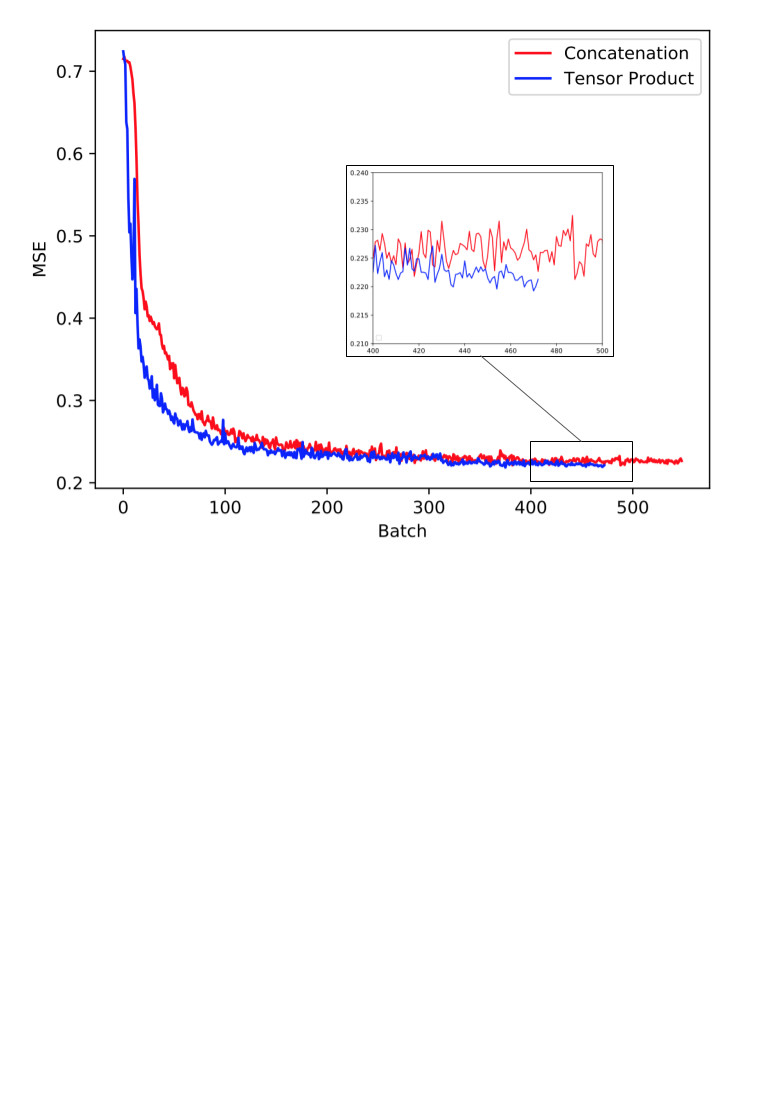
\includegraphics[trim={0 7.5in 0 0},clip,width=0.45\textwidth]{fig/Learning_curve.png}\label{fig:learning_curve}}
\subfloat[Correlation]{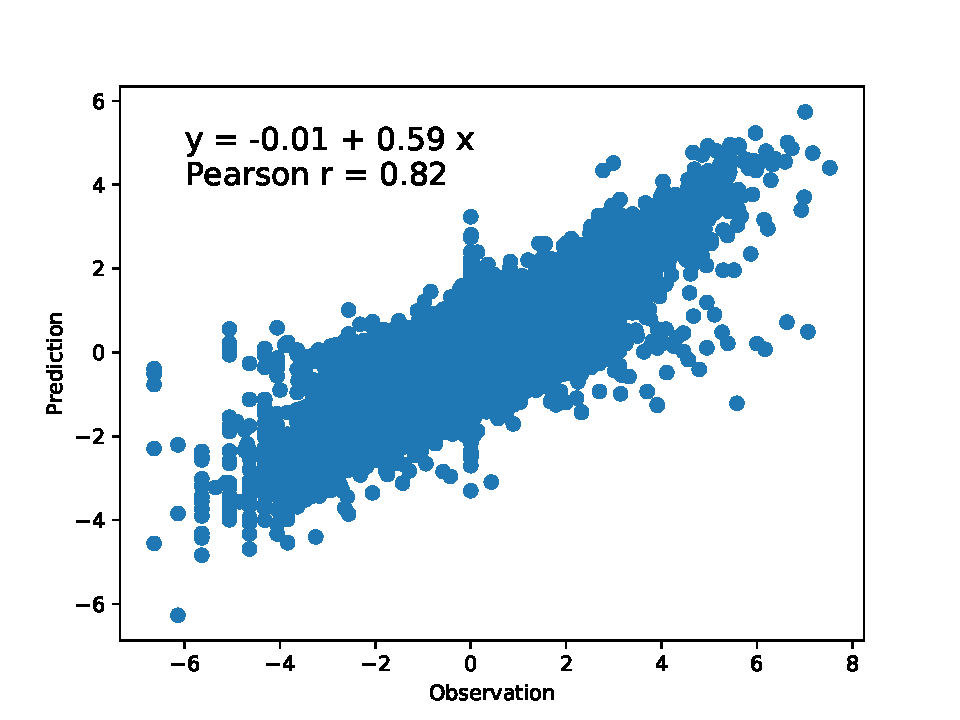
\includegraphics[trim={0.3in 0 0 0},clip,width=0.45\textwidth]{fig/correlation_tensor_product.pdf}\label{fig:correlation}}
\caption{Training and performance. (a) Validation error for concatenation and tensor product network. (b) Pearson correlation for tensor product network.}

\end{figure}


Compared with previous studies, all three architectures outperformed previous studies on the classification task. Our best model outperformed the previous best model by 16.6\% (Table \ref{table:classification performance}). 

\begin{table}[!hbt]
\caption{Classification performance}
\centering
 \begin{tabular}{|c | c|} 
 \hline
 Method & Accuracy \\
 \hline
 GeneClass & 60.9\% \\ 
 \hline
 BDTree & 62.9\% \\
 \hline
 DeepRAGE-C & \textbf{79.5\%} \\
 \hline
 DeepRAGE-TP & 77.0\% \\
 \hline
\end{tabular}
\label{table:classification performance}
\end{table}

\begin{table}[!hbt]
\caption{Confusion matrix}
\centering
 \begin{tabular}{|c | c c c|} 
 \hline
 {} & \multicolumn{3}{|l|}{Predicted by DeepRAGE-C} \\
  & Down & Baseline & Up \\ 
 \hline
 Down & 10.14 & 7.47 & 0.13 \\
 \hline
 Baseline & 3.29 & 59.77 & 3.02 \\
 \hline
 Up & 0.18 & 6.42 & 9.59 \\
 \hline
\end{tabular}
\label{table:confusion matrix}
\end{table}

\subsection{Recovering Known Motifs}
Discovering transcription factor binding motifs has been a central problem in computational biology. Existing models such as GeneClass and BDTree relies on existing motif annotations and lacks the ability to infer \textit{de novo} motif. Convolutional neural networks has the ability to learn filter weights and extracts motif information automatically. Studies have shown that known motifs can be recovered by CNNs trained on ChIP-seq data (\cite{Quang:2016jt,Kelley:2016bv,Alipanahi:2015fb}. In their settings, the training labels provide the model with direct evidence of which sequences are bound. In contrast, our model does not know which sequences are bound. Instead, the model needs to extract motifs common to genes that has similar expression profiles. Under the simplying assumption that all yeast promoter sequences are accessible to TFs, then similar motif structures would lead to similar expression patterns. We found that deepRAGE learns both known and \textit{de novo} motifs.

\begin{figure}[!tbp]
\centering

\subfloat{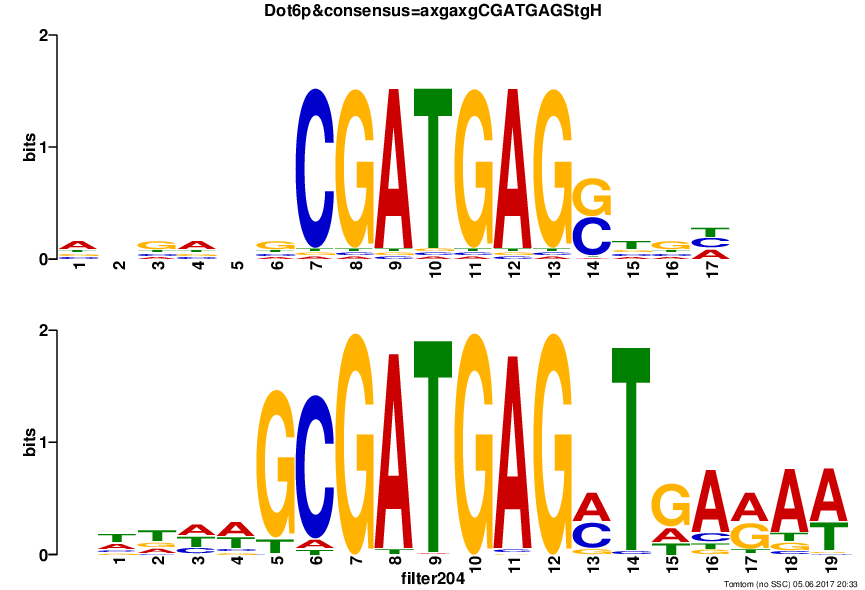
\includegraphics[width=0.2\textwidth]{fig/tomtom/dot6p_2.png}\label{fig:2a}}
\subfloat{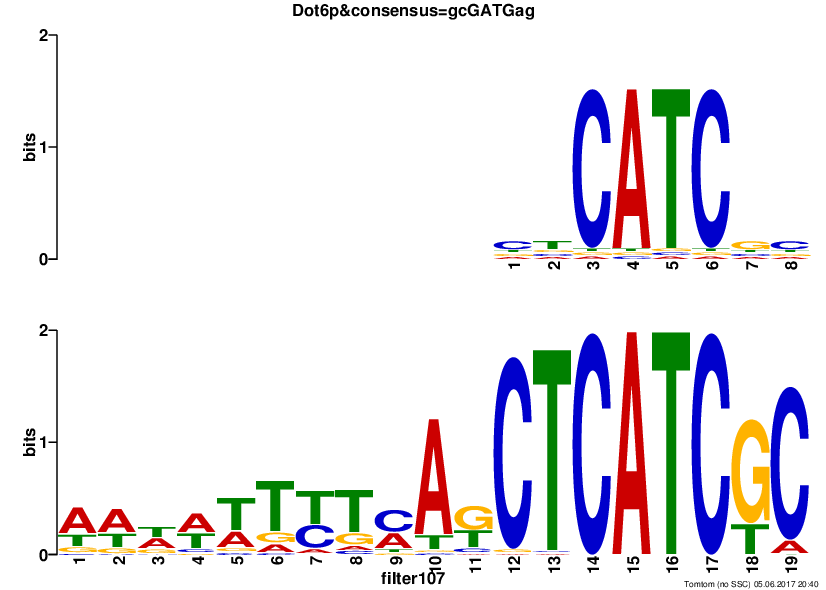
\includegraphics[width=.2\textwidth]{fig/tomtom/dot6p_3.png}\label{fig:2b}}
\subfloat{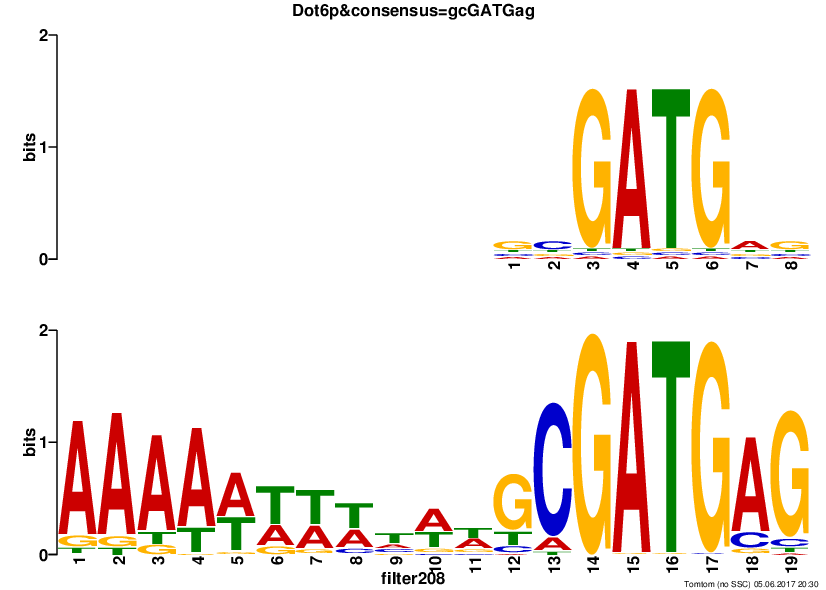
\includegraphics[width=.2\textwidth]{fig/tomtom/dot6p.png}\label{fig:2c}}
\subfloat{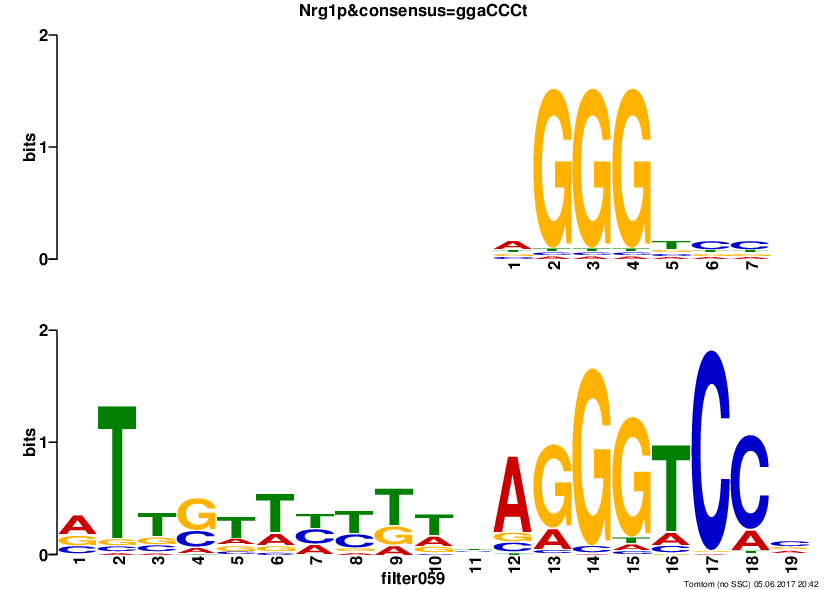
\includegraphics[width=.2\textwidth]{fig/tomtom/nrg1p.png}\label{fig:2d}}


\subfloat{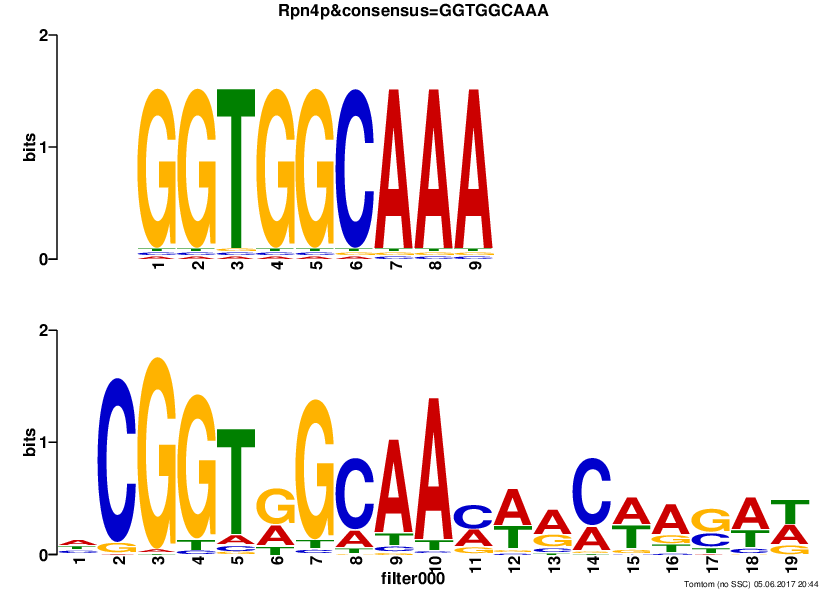
\includegraphics[width=.2\textwidth]{fig/tomtom/rpn4p.png}\label{fig:2e}}
\subfloat{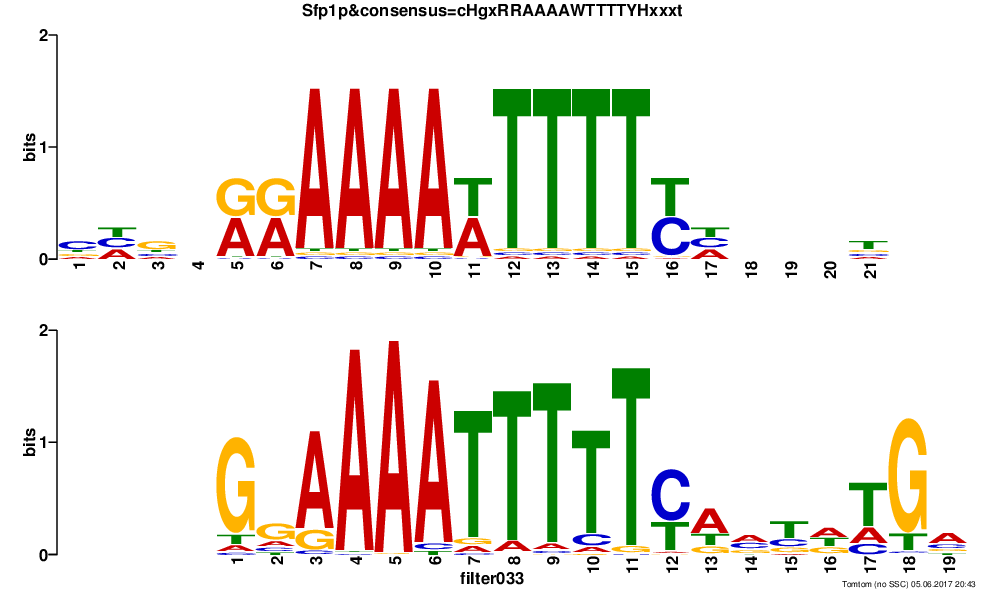
\includegraphics[width=.2\textwidth]{fig/tomtom/sfp1p_2.png}\label{fig:2f}}
\subfloat{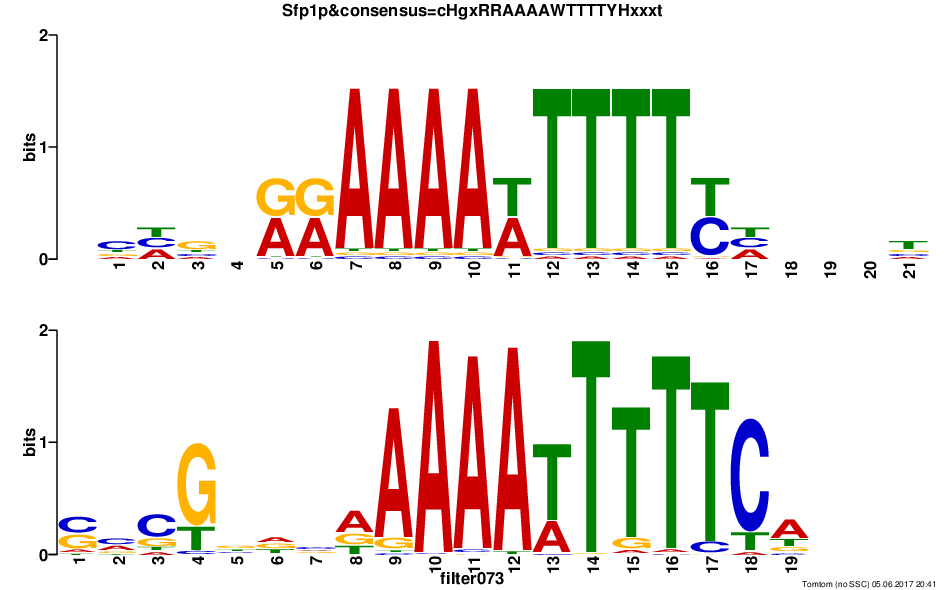
\includegraphics[width=.2\textwidth]{fig/tomtom/sfp1p.png}\label{fig:2g}}
\subfloat{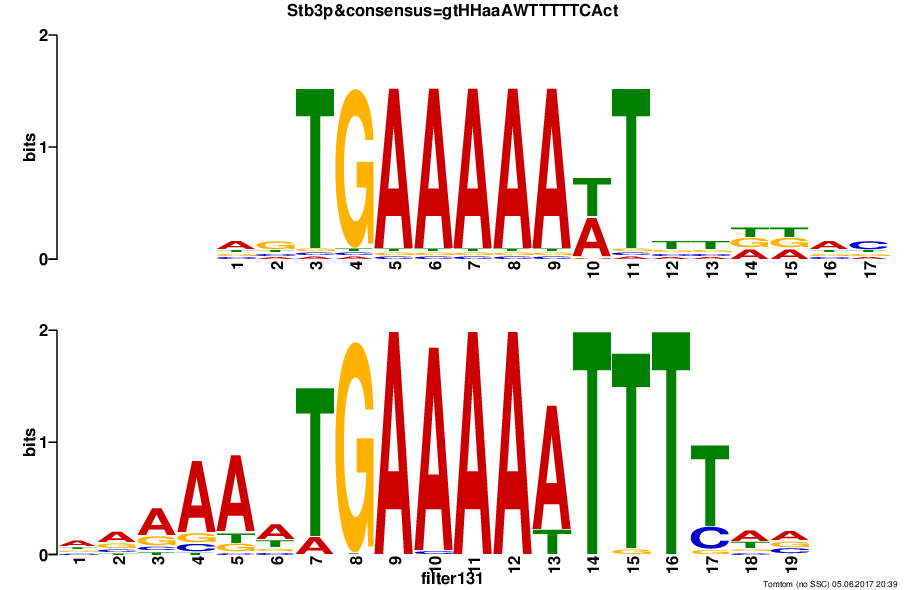
\includegraphics[width=.2\textwidth]{fig/tomtom/stb3p.png}\label{fig:2h}}

\caption{Example of known motifs recovered by the convolutional filters of deepRAGE}
\end{figure}

\subsection{Inferring gene-regulatory element relationships}

Our model allows us to infer the relationship between transcription factor and its potential target genes. As a proof of principal, we show that our model is able to link transcription factors and their target genes through known motifs. We first generated position weight matrices for each of the 256 filters from the first layer of the CNN by counting the frequence of nucleotide at each position from top 100 sequences with the highest activation. We queried against the YEASTRACT database for known motifs. Using a q-value cutoff of 0.1, 46 of 256 filters are matched for known motifs. We performed \textit{in silico} knockout experiments by setting the known motif weights to zeros. By comparing the predicted gene expression between the wild-type versus the knockout, we were able to infer the influence that motifs have on each gene. We validated whether the discovered TF-motif-gene relationship are reliable by comparing against annotation from the YEASTRACT database. For each TF-motif pair, we obtained a list of target genes, and calculate the absolute difference in predicted expression between the wild-type and the knockout. We find that the average change in expression were greater for annotated target genes than other genes (Wilcoxon rank-sum test p-value < 0.022).  

As an example, filter 164 matched to a canonical binding motif of Mig1p. After filter 164 is knocked out, three out of the top five genes with the largest expression changes are known targets of Mig1p (Fisher's exact test p-value < 0.0026). In addition, as Fig. \ref{mig1p} shows, most genes expression value stays unchanged after Mig1p has been knocked out, further indicating the specificity of our model. 

\begin{figure}
\center
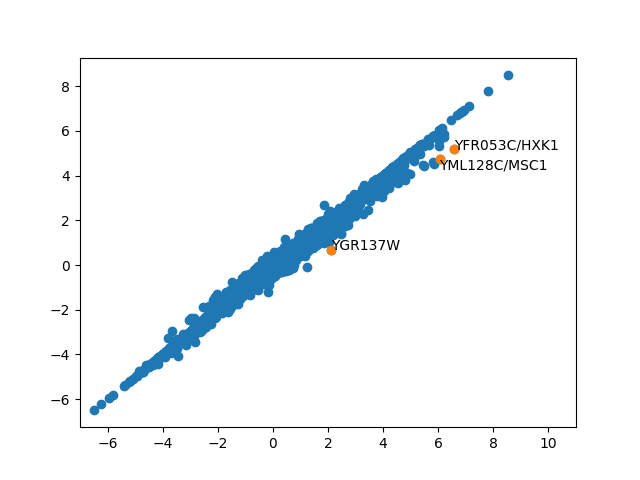
\includegraphics[width=0.5\textwidth]{fig/mig1p_filter164.png}
\caption{Prediction changes after knocking out Mig1p filter}
\label{mig1p}
\end{figure}


\section{Conclusion}

Deep learning has been widely applied in computational biology. In this work, we constructed a hybrid neural network that utilized both transcription factor abundance and sequence data to predict genome-wide gene expression value. We applied our model to yeast, a simple model organism whose regulatory circuitry has been extensively studied. Our model shows a 14-17\% increase over existing methods \textit{et al.} \cite{Kundaje:2007hs,Ruan:2006hl}. In addition, previous methods have all required known motif annotation, whereas our method does not. In fact, our model can automatically predict known motifs and, to a lesser extent, discover \textit{de novo} motifs. 

We experimented with two variants of deepRAGE and either has its own advantage. The concatenation network has smaller number of parameters and thus is faster to train. On the other hand, the tensor product network allows easier interpretation. In particular, it allows knocking out a specific motif-gene pair, which is not feasible within the concatenation framework. 
Using external annotations unknown during training, we show that our model recovers known TF-motif-gene relationship. As a proof-of-principle, we show that knocking out given motifs would influence the expression of known target genes. We envision that \textit{in silico} knockout experiment can assist in hypothesis generation, especially as a precursor to the more labor-intensive experimental screens. 

We believe that our model should be not restricted to model organisms. As opposed to the easy of manipulation for yeast, human studies are often much more time consuming and are under much stringent regulations. The ability to perform \textit{in silico} experiments would assist in hypothesis generation and therefore speed up experimental iterations. In the future, we would like to extend our model to human transcriptomic data. 


\bibliographystyle{unsrt}
\bibliography{references}


\end{document}
